\chapter{Numerical Results}

In this chapter the numerical results for this thesis will be presented. The first and section chapters conserns the verification and validation of the \textit{One-step $\theta$} scheme respectivly. In the third and final chapter, different speed-up strategies are presented and compared

\section{Verification}

\subsection{Fluid Problem}
One question which arises during the construction of the manufactured solution is, which formulation of the Navier-Stokes equation do we want to calculate the sourceterm. From a numerical point of view constructing the sourceterm from the Eulerian formulation and then map the equation would be feasable. Such an apporach limits the evaluation of computational demanding routines such as the generation of the deformation gradient $\hat{F}$ and its Jacobian $\ha{J}$. Even though refinement studies of spatial and temporal discretizations are often computed on small problems, such speed-ups are important when running larger simulations. 
Recall from Chapter ??? the ALE formulation of the Navier Stokes equation. 
\begin{align*}
&\rho_f \ha{J}\pder{\hat{u}}{t} + \ha{J} \hat{F}^{-1} (\hat{u} - \hat{w})\cdot \nabla \hat{u} 
- \nabla \cdot \ha{J} \sigma \hat{F}^{-T} = f \\
&\ha{div}(\ha{J}\hat{F}^{-1}\ha{u}) = 0
\end{align*}


%\begin{lstlisting}[style=python, frame=single, title=A Fibonaci example]
\begin{lstlisting}[style=python, caption={Descriptive Caption Text}, label=DescriptiveLabel, frame=single]
u_x = "cos(x[0])*sin(x[1])*cos(t_)"
u_y = "-sin(x[0])*cos(x[1])*cos(t_)"
p_c = "sin(x[0])*cos(x[1])*cos(t_)"

f = rho*diff(u_vec, t_) + rho*dot(grad(u_vec), (u_vec - w_vec)) -
div(sigma_f(p_c, u_vec, mu))
\end{lstlisting}

We will on the basis of the presented guidelines define the manufactured solution.

\begin{align*}
u = sin(x + y + t)^2 \\
v = cos(x + y +  t)^2 \\
p = cos(x + y + t)
\end{align*}

\newpage                                                                                                                                             

\section{Validation of a One-step $\theta$ scheme}
The numerical benchmark presented in \cite{Hron2006} has been chosen for validation of the \textit{One-step $\theta$} scheme presented in chapter. The benchmark has been widely accepted throughout the fluid-structure interaction community as a rigid validation benchmark. This is mainly due to the diversity of tests included, challenging all the main components of a fluid-structure interaction scheme. \\

The computational domain is based on the \textit{von Kármán vortex street} se (cite), where a cylinder is intentionally placed off center in a pipe. This configuration initiates a periodic shedding of vortices, as some fluid moves past the cylinder. In \cite{Hron2006}, an elastic flag is placed behind the cylinder. \\

\begin{figure}[h!]
  \centering
    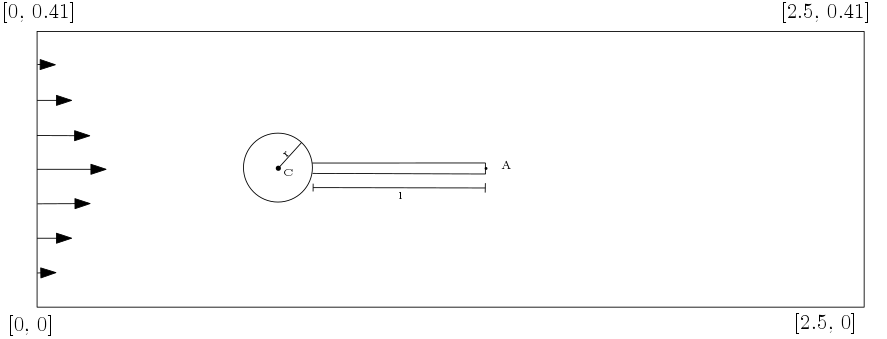
\includegraphics[scale=0.5]{./Fig/turekflag.png}
      \caption{Computational domain of the validation benchmark}
\end{figure}
\newpage


The benchmark is divided into three main test environments.
In the first environment the fluid solver is tested for a series of different flow profiles. \\
The second environment regards the structure implementation, regarding bending of the elastic flag. The third environment the full fluid-structure interaction problem.
The test environments are further divided into three different problems with increasing difficulty, posing different challenges to the implementation.

 Several quantites for comparion are presented in \cite{Hron2006} for validation purposes. The evaluation of these quantities are considered for fully developed flow,

\begin{itemize}
\item The position (x,y) of point A(t) as the elastic flag undergoes deformation.
\item Drag and lift forces exerted on of the whole interior geometry in contact with the fluid, consisting of the rigid circle and the elastic beam.
\begin{align*}
(F_D, F_L) = \int_{\Gamma} \mathbf{\sigma} \cdot \mathbf{n} dS
\end{align*}
\end{itemize}

The following environments and their sub-problems presents both steady state and periodic solutions. For the steady state solutions, the quantity of interest will be calculated for the last timestep. For the periodic solutions, the amplitude and mean values for the time dependent quantity are calculated from the last period of oscillations.The mean value and amplitude is given by,
\begin{align*}
\text{mean} = \frac{1}{2} \text{max + min} \\
\text{amplitude} = \frac{1}{2} \text{max . min}
\end{align*}
from the maximum and minimum value of the quantity of interest from the last period.  

 In \cite{Hron2006}, all steady state solutions seems to be calulated by solving a steady state equation such as the stokes equation for the fluid problem. The assumtion is based on simulation paramters regarding time-step are only reported for the periodic solutions. In this thesis all problems in \cite{Hron2006},will be calculated by time integration. The main motivation is based upon that any given numerical errors regarding time integration will be intercepted at an earlier stage for a simpler problem. Therefore, the choice of timestep  is chosen such that reasonable accuracy of the reference solution is attained.

In \cite{Hron2006}, details such as  finite-element spaces and newton iteration critera are not reported. Therefore, the following numerical results have been a process of trial and error. In the following section, an overview of each environment togheter with  the numerical results will be presented. A formal discussion of the results are given at the end of each simulation environment. For each table, the error of the finest spatial and temporal refinement compared to the reference solution is reported .

 Since the first two simulation environmens are presented mainly in support of the third and final environment, they where not reported in OTHER CITE. Therefore results in the first two subsections  will be compared with \cite{Hron2006}, while the third will consider both \cite{Hron2006} and OTHER CITE.

 \newpage
\subsection{Validation of fluid solver}
The first test environment conserns the fluid dynamics part of the total FSI problem, to ensure the solver can handle flows in low Reynold-numbers regime. Two approaches for the validation are given in \cite{Hron2006}. The first approach consideres setup as a fluid-structure interaction problem, by setting the elastic flag close to rigid  by manipulation of the structure paramters. Second, the flag can be set fully rigid and considered a purly flow problem.  Hence, the fluid variation formulation can be reduced to


Find $\bat{v}_f, \ha{p}_f $ such that
\begin{align*}
 \big( \pder{\bat{v}}{t}, \ \gat{\psi}^u \big)_{\hat{\Omega}_f} +
\femf{(\bat{v} \cdot \hat{\nabla}) \bat{v}}{\gat{\psi}^u}
- \femf{\hat{\sigma}}{\hat{\nabla}\gat{\psi}^u} -
\femf{\rho_f  \mathbf{f}_f}{{\gat{\psi}^u}} = 0 \\
\femf{\nabla \cdot \bat{v})}{\gat{\psi}^p} = 0 
\end{align*} 

The latter approach is chosen for this thesis, as only the variational formulation for the fluid is tested and removes any influence of the strucutre and mesh extrapolation discretization.  Since $\hat{\Omega}_f = {\Omega}_f(t) \hspace{2mm} t \in T$, the mesh velocity of the fluid $ \pder{\ha{T}_W}{t} = 0$  and no deformation of the fluid domain is present.

The validation of the fluid solver is divided into the three sub-cases CFD1, CFD2 and CFD3.While  CFD1 and CFD2 yields steady state solutions, CFD3 is a periodic solution.

%\begin{figure}[h!]
  %\centering
    %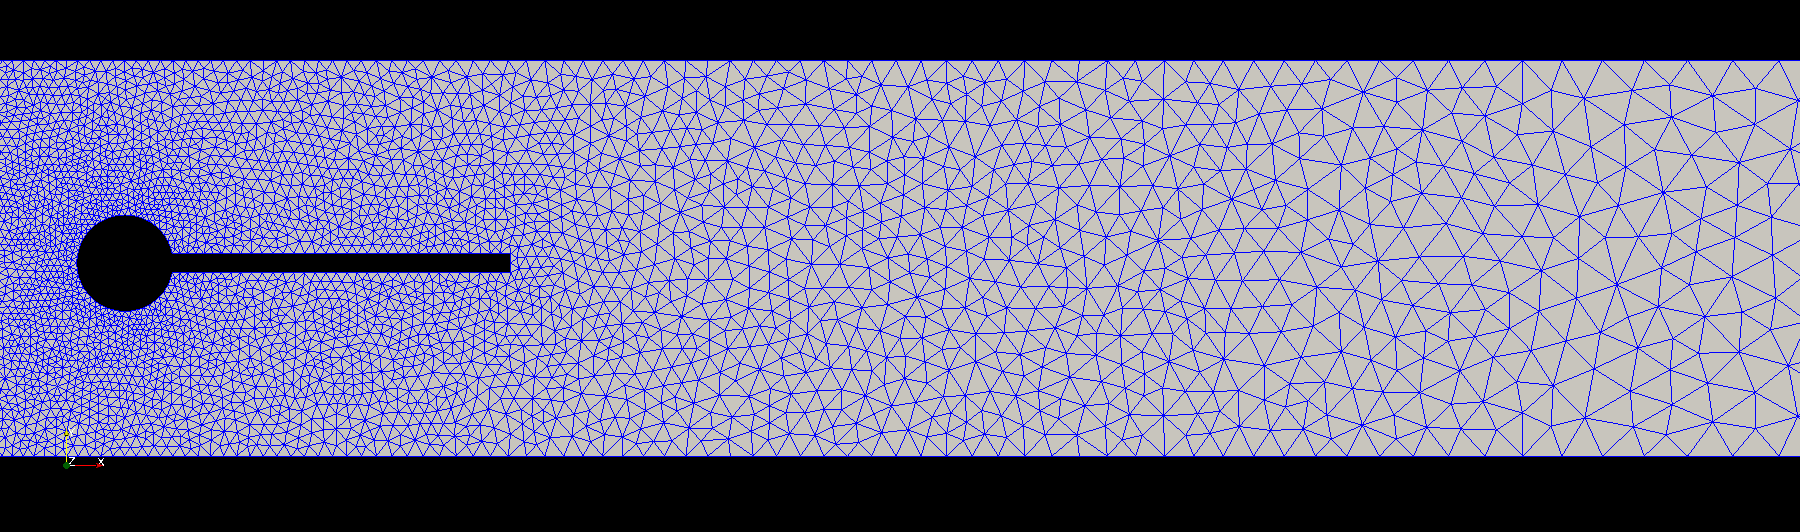
\includegraphics[scale=0.3]{./Fig/cfd1mesh.png}
      %\caption{Computational domain of channel flow with rigid inner geometry. }
%\end{figure}

\begin{table}[h!]
\centering
\caption{Benchmark environment}
\label{my-label}
\begin{tabular}{ |p{3cm}||p{2cm}|p{2cm}|p{2cm}|  }
 \hline
 \multicolumn{4}{|c|}{Fluid parameters} \\
 \hline
 parameter              & CFD 1 & CFD 2 & CFD 3 \\
 \hline
$\rho^f [10^{3}\frac{kg}{m^3}]$ & 1    & 1    & 1    \\
$\nu^f  [10^{-3}\frac{m^2}{s}]$  & 1    & 1    & 1    \\
U                      & 0.2  & 1    & 2    \\
Re                     & 20   & 100  & 200 \\
\hline
\end{tabular}
\end{table}

A parabolic velocity profile on the form,
\begin{align*}
v_f(0, y) = 1.5 U\frac{(H -y)y}{(\frac{H}{2})^2}
\end{align*}
is set on the left channel inflow. H is the height of the channel, while the parameter U is set differently to each problem to induce different flow profiles. \

At the right channel outflow, the pressure is set to $p = 0$. \
No-slip boundary conditions for the fluid are enforced on the channel walls, and on the inner geometry consisting of the circle and the elastic flag.
The validation is based on the evaluation of drag and lift forces on the inner geometry for each sub-case.  with comparison to \cite{Hron2006}. Each sub-case will be conducted on four different mesh, with increasing refinement.  The following tables presents the numerical results for each sub-case.

\newpage

\begin{table}[h!]
\centering
\caption{CFD 1 Results}
\label{CFD 1 Results}
\begin{tabular}{ |p{1cm}||p{2.7cm}|p{3.3cm}|p{3.3cm}|}
\hline
  \multicolumn{4}{|c|}{$\Delta t = 0.1 \hspace{2mm} \theta = 1.0$} \\
\hline
nel & ndof & Drag  & Lift \\
\hline
 1438    & 6881   & 13.60 & 1.089  \\
 2899    & 13648  & 14.05 & 1.126 \\
 7501    & 34657  & 14.17   & 1.109 \\
 19365   & 88520  & 14.20 & 1.119 \\
  \hline
  \multicolumn{2}{|c|}{Reference}  & 14.29   & 1.119\\
   \hline
    \multicolumn{2}{|c|}{Error}  & 0.006 \%   & 0.00 \%\\
   \hline
\end{tabular}
\end{table}

\begin{table}[h!]
\centering
\caption{CFD-2}
\label{CFD-2 Results}
\begin{tabular}{ |p{1cm}||p{2.7cm}|p{3.3cm}|p{3.3cm}|}
 \hline
  \multicolumn{4}{|c|}{$\Delta t = 0.01 \hspace{2mm} \theta = 1.0$} \\
   \hline
nel & ndof & Drag  & Lift \\
\hline
 1438    & 6881 (P2-P1)  & 126.0 &  8.62 \\
 2899    & 13648  (P2-P1)& 131.8 & 10.89  \\
 7501    & 34657 (P2-P1) & 135.1 & 10.48  \\
 19365   & 88520(P2-P1)  & 135.7 & 10.55  \\
 \hline
  \multicolumn{2}{|c|}{Reference}  & 136.7   & 10.53\\
   \hline
    \multicolumn{2}{|c|}{Error}  & 0.007 \%   & 0.001 \%\\
   \hline
\end{tabular}
\end{table}

\begin{figure}[h!]
  \centering
    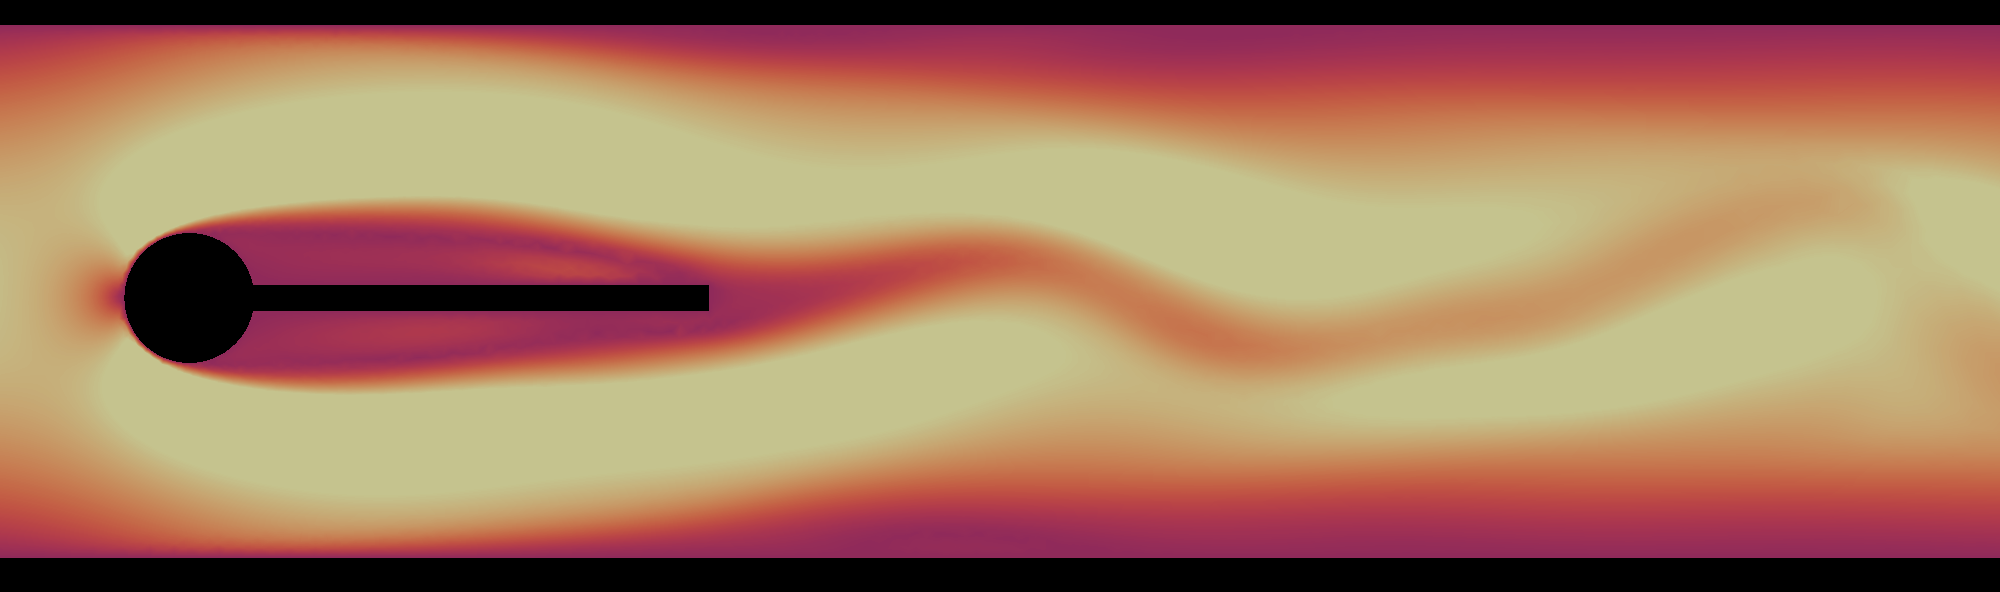
\includegraphics[scale=0.2]{./Fig/cfd3.png}
      \caption{CFD-3, flow visualization of velocity time t = 9s}
\end{figure}

\begin{figure}[h!]
  \centering
    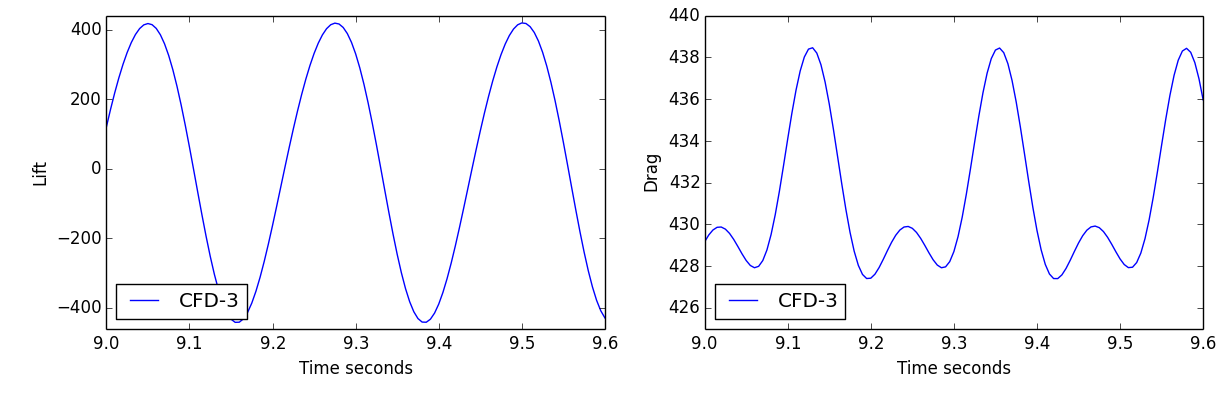
\includegraphics[scale=0.5]{./Fig/cfd3_liftdrag.png}
      \caption{CFD-3, lift and drag forces at time t = [9, 9.6]}
\end{figure}


\begin{table}[h!]
\centering
\caption{CFD-3}
\label{CFD-3 Results}
\begin{tabular}{ |p{1cm}||p{2.9cm}|p{3.3cm}|p{3.3cm}|}
 \hline
  \multicolumn{4}{|c|}{$\Delta t = 0.01 \hspace{2mm} \theta = 0.5$} \\
   \hline
nel & ndof & Drag  & Lift \\
\hline
 1438    & 6881  (P2-P1)   & 417.23       +/-  0.0217 & -249.21       +/-  0.32  \\
   & 16474 (P3-P2)   & 414.86      $\pm$  5.6282 & -7.458      $\pm$  444.07  \\
 \hline
 2899    & 13648  (P2-P1) & 408.50  $\pm$   4.3029 & -19.731  $\pm$   373.45 \\  
     &  32853 (P3-P2)  & 432.86      $\pm$  5.5025 & -9.686      $\pm$  431.28  \\
  \hline
  7501    & 34657 (P2-P1) & 431.57  $\pm$   5.2627 & -12.497  $\pm$   429.76 \\    
    &  83955 (P3-P2)  & 438.20      $\pm$  5.5994 & -11.595      $\pm$  438.00 \\
    \hline
    19365   & 88520 (P2-P1) & 435.43  $\pm$   5.4133 & -11.545  $\pm$   438.89 \\
   &   215219 (P3-P2) & 438.80      $\pm$  5.6290 & -11.158      $\pm$  439.23 \\
\hline
 \multicolumn{2}{|c|}{Reference}  & 439.95 $\pm$ 5.6183 & -11.893 $\pm$ 437.81\\
 \hline
  \multicolumn{2}{|c|}{Error}  & 0.002 \% $\pm$ 0.001 \% & 0.061 \% $\pm$ 0.003\% \\
  \hline
  \end{tabular}
  \vspace{2cm}
 \begin{tabular}{ |p{1cm}||p{2.9cm}|p{3.3cm}|p{3.3cm}|}
  \hline
  \multicolumn{4}{|c|}{$\Delta t = 0.005 \hspace{2mm} \theta = 0.5$} \\
   \hline
nel & ndof & Drag  & Lift \\
\hline
 1438    & 6881  (P2-P1)   &  417.24  $\pm$  0.0084 & -249.386   $\pm$ 0.1345  \\
 1438    & 16474 (P3-P2)   & 414.90     $\pm$  5.7319 & -8.467 $\pm$  443.45  \\
\hline
 1438    &13648  (P2-P1)   & 408.27   $\pm$ 4.0192 & -18.981   $\pm$ 363.84 \\
 2899    &  32853 (P3-P2)   & 432.90      $\pm$  5.5333 & -11.382      $\pm$  430.60 \\
 \hline
 1438    & 34657  (P2-P1)   & 431.59 $\pm$5.2979 & -13.644   $\pm$ 429.68 \\
 7501    & 83955 (P3-P2)  & 438.23      $\pm$  5.6393 & -12.917 $\pm$  437.78 \\
 \hline
 1438    & 88520  (P2-P1)   & 435.46  $\pm$ 5.4579 & -13.190   $\pm$ 438.05 \\
 19365   & 215219 (P3-P2)  & 438.84    $\pm$  5.6576 & -12.786      $\pm$  438.36 \\
\hline
 \multicolumn{2}{|c|}{Reference}  & 439.95 $\pm$ 5.6183 & -11.893 $\pm$ 437.81\\
 \hline
  \multicolumn{2}{|c|}{Error}  & 0.002 \% $\pm$ 0.006 \% & 0.075 \% $\pm$ 0.001\% \\
  \hline
\end{tabular}
\end{table}

\newpage \newpage \newpage \newpage \newpage
\subsection{Discussion of results}
The numerical results for CFD1, CFD2 and CFD3 are all within reasonable range of the reference solutions presented in \cite{Hron2006}. 
For CFD1 and CFD2, the choice of P2-P1 elements together with a fully implicit schene $\theta = 1$ gained sufficient accuracy in comparison with the reference solution. The second order cranc-nicholoson scheme  $\theta = 0.5$ was investigated for CFD1 and CFD2, however only improving the results of order $10^{-6}$ for both lift and drag. For the periodic problem CFD-3, the choice of  P2-P1 elements with a fully implicit time-stepping scheme proved unsuficcient for capturing the expected periodic solution. Only a steady-state flow profile was observed.. By cranc-nicolson time-stepping scheme $\theta = 0.5$, the periodic solution was attained. Since the choice of finite-elemt pair is not reported in the original work, both P3-P2 and P2-P1 element pairs for fluid and pressure repsectivly was compared in combination with spatial mesh refinement. From Table 1.4, the choice P3-P2 element pair is eminent to achieve reasonable results for the first and second mesh regardless of timestep.  However, the third and fourth mesh shows close resemblance with the reference solution. \\
On this basis, the choice of P2-P1 element pair is sufficient for the evaluation of drag and lift on the inner geometry with increasing mesh resolution. 

\newpage
\subsection{Validation of solid solver}
\begin{table}[h!]
\centering
\caption{CSM validation environment}
\label{my-label}
\begin{tabular}{ |p{3cm}||p{2cm}|p{2cm}|p{2cm}|  }
 \hline
 \multicolumn{4}{|c|}{Fluid parameters} \\
 \hline
 parameter              & CSM 1 & CSM 2 & CSM 3 \\
 \hline
$\rho^s [10^{3}\frac{kg}{m^3}]$ & 1    & 1    & 1    \\
$\nu^s $  & 0.4    & 0.4    & 0.4    \\
$\mu^s  [10^{6}]$  & 0.5    & 2.0    & 0.5    \\

\hline
\end{tabular}
\end{table}

The validation of the solid solver are conducted on three refined mesh, where the number of elements are chosen in close resemblance with the original work in \cite{Hron2006}. A simple investigation of different finite-element pairs, suggest that P3-P3 elements where used for making the reference solution. In this study, lower order finite-element pair was included by the motivation of shorter simulation time while retaining solution accuracy. While computational time is not a major concern for the solid solver, the study is important for potentially reducing the computational time for the FSI-solver.ß

\begin{table}[h!]
\centering
\caption{CSM 1 Results}
\label{CSM 1 Results}
\begin{tabular}{ |p{1cm}||p{2.7cm}|p{3.3cm}|p{3.3cm}|}
\hline
  \multicolumn{4}{|c|}{$\Delta t = 0.1 \hspace{2mm} \theta = 1.0$} \\
\hline
nel & ndof & ux of A [x $10^{3}$]  &uy of A [x $10^{3}$] \\
\hline
 319     & 832 P1-P1  & -5.278 &  -56.6 \\
     & 2936 P2-P2 & -7.056 &  -65.4 \\
      & 6316 P3-P3 &  -7.064 &   -65.5  \\
 \hline
  1365    & 3140 P1-P1  & -6.385 &  -62.2 \\
     & 11736 P2-P2 & -7.075 &  -65.5 \\
     & 25792 P3-P3 & -7.083 &  -65.5 \\
 \hline
  5143    & 11084 P1-P1 & -6.905 &  -64.7  \\
     & 42736 P2-P2 & -7.083 &  -65.4\\
     & 94960 P3-P3 & -7.085 &  -65.5  \\
  \hline
  \multicolumn{2}{|c|}{Reference}  &-7.187    & -66.1 \\
   \hline
    \multicolumn{2}{|c|}{Error}  & 1.41 \%   & 0.8 \%\\
   \hline
\end{tabular}
\end{table}

\begin{table}[h!]
\centering
\caption{CSM 2 Results}
\label{CSM 2 Results}
\begin{tabular}{ |p{1cm}||p{2.7cm}|p{3.3cm}|p{3.3cm}|}
\hline
  \multicolumn{4}{|c|}{$\Delta t = 0.05 \hspace{2mm} \theta = 1.0$} \\
\hline
nel & ndof & ux of A [x $10^{3}$]  &uy of A [x $10^{3}$] \\
\hline

 319     & 832 P1-P1  & -0.3401 &  -14.43  \\ 
     & 2936 P2-P2 &  -0.460  &  -16.78  \\ 
      & 6316 P3-P3 & -0.461 &  -16.79  \\
        \hline
  1365    & 3140 P1-P1  &  -0.414 &  -15.93\\
     & 11736 P2-P2 &  -0.461 &  -16.81 \\
     & 25792 P3-P3 & -0.461  &  -16.82 \\
        \hline
   5143    & 11084 P1-P1 & -0.449 &  -16.60  \\
     & 42736 P2-P2 &-0.461 &  -16.82 \\
     & 94960 P3-P3 & -0.462 &  -16.82 \\
  \hline
  \multicolumn{2}{|c|}{Reference}  & -0.469      & -16.97  \\
   \hline
    \multicolumn{2}{|c|}{Error}  & 1.49\%   & 0.88 \%\\
   \hline
\end{tabular}
\end{table}

\begin{table}[h!]
\centering
\caption{CSM 3 Results}
\label{CSM 3 Results}
\begin{tabular}{ |p{1cm}||p{2.7cm}|p{3.3cm}|p{3.3cm}|}
\hline
  \multicolumn{4}{|c|}{$\Delta t = 0.02 \hspace{2mm} \theta = 0.5$} \\
\hline
nel & ndof & ux of A [x $10^{3}$]  &uy of A [x $10^{3}$] \\
\hline
 319     & 832 P1-P1  & -10.790       +/-  10.797 & -55.184       +/-  56.682 \\
     & 2936 P2-P2 & -14.380       +/-  14.387 & -63.198       +/-  65.147 \\
      & 6316 P3-P3 & -14.409       +/-  14.417 & -63.288       +/-  65.225 \\
  \hline
   1365    & 3140 P1-P1 & -13.032       +/-  13.041 & -60.446       +/-  62.075 \\
     & 11736 P2-P2 & -14.407       +/-  14.416 & -63.283       +/-  65.220 \\
     & 25792 P3-P3 & -14.412       +/-  14.421 & -63.310       +/-  65.246 \\
   \hline
    5143    & 11084 P1-P1 & -14.059       +/-  14.071 & -62.591       +/-  64.473 \\
     & 42736 P2-P2  & -14.412       +/-  14.421 & -63.313       +/-  65.249 \\
     & 94960 P3-P3 & -14.416       +/-  14.425 & -63.328       +/-  65.263 \\
    \hline
  \multicolumn{2}{|c|}{Reference}  &-14.305 +- -14.305        & -63.607 +- 65.160    \\
   \hline
    \multicolumn{2}{|c|}{Error}  & \%   &  \%\\
   \hline
\end{tabular}
\end{table}

\begin{table}[h!]
\centering
%\caption{CSM 3 Results 2}
\label{CSM 3 Results 2}
\begin{tabular}{ |p{1cm}||p{2.7cm}|p{3.3cm}|p{3.3cm}|}
\hline
  \multicolumn{4}{|c|}{$\Delta t = 0.01 \hspace{2mm} \theta = 0.5$} \\
\hline
nel & ndof & ux of A [x $10^{3}$]  &uy of A [x $10^{3}$] \\
\hline
    319     & 832 P1-P1 & -10.835       +/-  10.836 & -55.197       +/-  56.845 \\
     & 2936 P2-P2 & -14.390       +/-  14.392 & -63.303       +/-  65.149 \\
      & 6316 P3-P3& -14.432       +/-  14.435 & -63.397       +/-  65.263 \\
    \hline
    1365    & 3140 P1-P1  & -13.053       +/-  13.054 & -60.367       +/-  62.241 \\
     & 11736 P2-P2  & -14.428       +/-  14.432 & -63.388       +/-  65.256 \\
     & 25792 P3-P3  & -14.444       +/-  14.446 & -63.432       +/-  65.287 \\
     \hline
     5143    & 11084 P1-P1 & -14.082       +/-  14.084 & -62.656       +/-  64.495 \\
     & 42736 P2-P2 & -14.444       +/-  14.447 & -63.435       +/-  65.288 \\
     & 94960 P3-P3& -14.449       +/-  14.452 & -63.449       +/-  65.296 \\
 \hline
  \multicolumn{2}{|c|}{Reference}  &-14.305 +- -14.305        & -63.607 +- 65.160    \\
   \hline
    \multicolumn{2}{|c|}{Error}  & \%   &  \%\\
   \hline
\end{tabular}
\end{table}


\begin{table}[h!]
\centering
%\caption{CSM 3 Results 3}
\label{CSM 3 Results 3}
\begin{tabular}{ |p{1cm}||p{2.7cm}|p{3.3cm}|p{3.3cm}|}
\hline
  \multicolumn{4}{|c|}{$\Delta t = 0.005 \hspace{2mm} \theta = 0.5$} \\
\hline
nel & ndof & ux of A [x $10^{3}$]  &uy of A [x $10^{3}$] \\
\hline
    319     & 832 P1-P1 & -10.846       +/-  10.848 & -56.049       +/-  56.053 \\
     & 2936 P2-P2  & -14.390       +/-  14.391 & -63.738       +/-  64.703 \\
      & 6316 P3-P3 & -14.429       +/-  14.430 & -63.833       +/-  64.810 \\
 \hline 
    1365    & 3140 P1-P1 & -13.057       +/-  13.057 & -60.813       +/-  61.826 \\
     & 11736 P2-P2& -14.426       +/-  14.427 & -63.827       +/-  64.801 \\
     & 25792 P3-P3 & -14.440       +/-  14.441 & -63.854       +/-  64.845 \\
 \hline
      5143    & 11084 P1-P1 & -14.091       +/-  14.091 & -63.195       +/-  63.981 \\
     & 42736 P2-P2 & -14.441       +/-  14.441 & -63.856       +/-  64.847 \\
     & 94960 P3-P3 & -14.446       +/-  14.446 & -63.865       +/-  64.860 \\
 \hline
  \multicolumn{2}{|c|}{Reference}  &-14.305 +- -14.305        & -63.607 +- 65.160    \\
   \hline
    \multicolumn{2}{|c|}{Error}  & \%   &  \%\\
   \hline
\end{tabular}
\end{table}

\begin{figure}[h!]
  \centering
    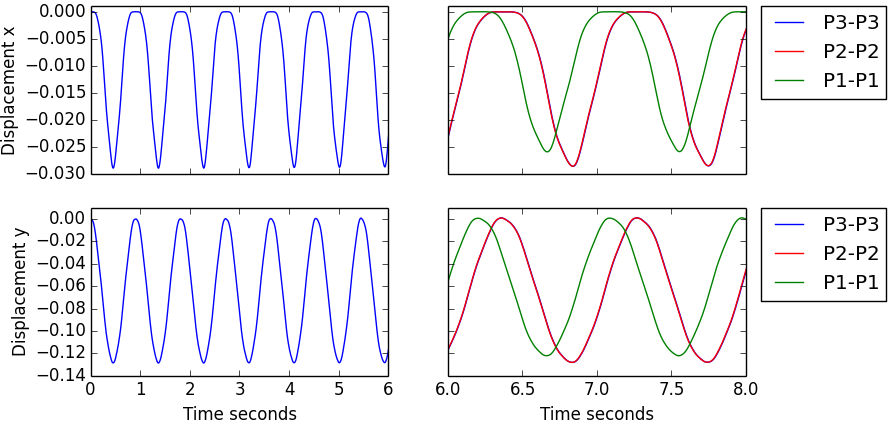
\includegraphics[scale=0.6]{./Fig/csm3compare.png}
      \caption{CSM-3, deformation components of A(t) for two different time intervals. Time interval $t \in [0, 6]$ shows the P3-P3 element pair, while$t \in [6, 8]$ compares all finite elemet pair chosen for the experiment}
\end{figure}

\subsection{Discussion of results}
The results for sub-problems CSM-1 and CSM-2 each coincide with the reference solution. The study of lower-grade elements proved successful for both problems, justifying accurate results can be achieved for polynomials grade 1 and 2 for all mesh refinements. This obeservation is furhter justified in the CSM-3 reults. In table 1.4, the  displacement components of P3-P3 and P2-P2 elements can hardly be distinguished.


\newpage
\subsection{Validation of fluid structure interaction solver}
The validation of the FSI solver constist of three sub-cases which will be referred to FSI-1, FSI-2 and FSI-3. The FSI-1 environment yields a steady state solution for the system, inducing small deformations to the elastic flag. This environment is exelent to ensure the overall coupling of the FSI-problem is exectuted properly. The FSI-2 and FSI-3 environment results in a periodic solution, where the elastic flag oscilates behind the sylinder.


 For all sub-cases
a parabolic velocity profile on the form,
\begin{align*}
v_f(0, y) = 1.5 U\frac{(H -y)y}{(\frac{H}{2})^2}
\end{align*}
is set on the left channel inflow. H is the height of the channel, while the parameter U is set differently to each problem to induce different flow profiles. \
At the right channel outflow, the pressure is set to $p = 0$. \
No-slip boundary conditions for the fluid are enforced on the channel walls, and on the circle of the inner geometry.
The structure deformation and velocity is set to zero on the left side of the flag, where the flag is ancored to the circle. On the fluid-structure interface $\Gamma$, we enfore the kinematic and dynamic boundary condition
\begin{align}
\mathbf{v}_f = \mathbf{v}_s \\
\mathbf{\sigma}_f \cdot \mathbf{n} = \mathbf{\sigma}_s \cdot \mathbf{n}
\end{align}
From chapter ?,  (1.1) is enforced strongly due to the continious velocity field, while (1.2) is enforced weakly by omtitting form the weak formulation by.



Apart from the accuracy of the reported values, the main purpose of the validation of the fluid solver is twofold. Firstly, it is of great importance to ensure that the overall coupling of the fluid-structure interaction problem are executed correctly. Second, a good choice of mesh extrapolation model is essential to ensure that mesh entanglement is not present. Based on the experience with the previous sub-problems, the finite element group of P2-P2-P1 is chosen for deformation, velocity and pressure respectivly. 


\begin{table}[h!]
\centering
\caption{Benchmark environment}
\label{my-label}
\begin{tabular}{ |p{3cm}||p{2cm}|p{2cm}|p{2cm}|  }
 \hline
 \multicolumn{4}{|c|}{Solid parameters} \\
 \hline
 parameter              & FSI1 & FSI2 & FSI3 \\
 \hline
 $\rho^s [10^{3} \frac{kg}{m^3}]$ & 1    & 10   & 1    \\
$\nu^s$ & 0.4  & 0.4  & 0.4  \\
$\mu^s  [10^{6}\frac{kg}{ms^2}]$  & 0.5  & 0.5  & 2.0  \\
 \hline
 \multicolumn{4}{|c|}{Fluid parameters} \\
 \hline
$\rho^f [10^{3}\frac{kg}{m^3}]$ & 1    & 1    & 1    \\
$\nu^f  [10^{-3}\frac{m^2}{s}]$  & 1    & 1    & 1    \\
U                      & 0.2  & 1    & 2    \\
parameter              & FSI1 & FSI2 & FSI3 \\
Re                     & 20   & 100  & 200 \\
\hline
\end{tabular}
\end{table}

\newpage
\subsubsection{FSI1}


\begin{table}[h!]
\centering
\caption{FSI 1 Results}
\label{FSI1 Results}
\begin{tabular}{ |p{1cm}||p{1cm}|p{2.5cm}|p{2.5cm}|p{2.7cm}|p{2.7cm}|p{1.2cm}|}
 \hline
  \multicolumn{6}{|c|}{Laplace} \\
   \hline
nel & ndof & ux of A [x $10^{3}$]  &uy of A [x $10^{3}$]& Drag  & Lift \\
 \hline
 2474    & 21249  &       0.0226 &       0.8200 & 14.061 & 0.7542 \\
 7307    & 63365  &       0.0227 &       0.7760 & 14.111 & 0.7517 \\
 11556   & 99810  &       0.0226 &      0.8220 & 14.201 & 0.7609 \\
  \hline
 \multicolumn{2}{|c|}{Reference} &  0.0227      &       0.8209      & 14.295  & 0.7638   \\
 \hline
\end{tabular}
\begin{tabular}{ |p{1cm}||p{1cm}|p{2.5cm}|p{2.5cm}|p{2.7cm}|p{2.7cm}|p{1.2cm}|}
 \hline
  \multicolumn{6}{|c|}{Linear Elastic} \\
   \hline
nel & ndof & ux of A [x $10^{3}$]  &uy of A [x $10^{3}$]& Drag  & Lift \\
 \hline
 2474    & 21249  &       0.0226 &       0.8198 & 14.061 & 0.7541 \\
 7307    & 63365  &       0.0227 &       0.7762 & 14.111 & 0.751  \\
 11556   & 99810  &       0.0226  &       0.8222 & 14.201 & 0.7609 \\
  \hline
 \multicolumn{2}{|c|}{Reference} &  0.0227      &       0.8209      & 14.295  & 0.7638   \\
 \hline
\end{tabular}
\begin{tabular}{ |p{1cm}||p{1cm}|p{2.5cm}|p{2.5cm}|p{2.7cm}|p{2.7cm}|p{1.2cm}|}
 \hline
  \multicolumn{6}{|c|}{Biharmonic bc1} \\
   \hline
nel & ndof & ux of A [x $10^{3}$]  &uy of A [x $10^{3}$]& Drag  & Lift \\
 \hline
 2474    & 21249  &       0.0226 &       0.8200 & 14.061 & 0.7541 \\
 7307    & 63365  &       0.0227  &       0.7761 & 14.111 & 0.7517 \\
 11556   & 99810  &       0.0227  &       0.8017 & 14.205 & 0.9248 \\
  \hline
 \multicolumn{2}{|c|}{Reference} &  0.0227      &       0.8209      & 14.295  & 0.7638   \\
 \hline
\end{tabular}
\begin{tabular}{ |p{1cm}||p{1cm}|p{2.5cm}|p{2.5cm}|p{2.7cm}|p{2.7cm}|p{1.2cm}|}
 \hline
  \multicolumn{6}{|c|}{Biharmonic bc2} \\
   \hline
nel & ndof & ux of A [x $10^{3}$]  &uy of A [x $10^{3}$]& Drag  & Lift \\
 \hline
 2474    & 21249  &       0.0226 &       0.8200 & 14.061 & 0.7543 \\
 7307    & 63365  &       0.0227 &       0.7761 & 14.111 & 0.7518 \\
 11556   & 99810  &       0.0227 &       0.8020 & 14.205 & 0.9249  \\
  \hline
 \multicolumn{2}{|c|}{Reference} &  0.0227      &       0.8209      & 14.295  & 0.7638   \\
 \hline
\end{tabular}
\end{table}


\begin{table}[h!]
\centering
\caption{FSI 1 - No extrapolation}
\label{FSI1- No extrapolation}
\begin{tabular}{ |p{1cm}||p{1cm}|p{2.5cm}|p{2.5cm}|p{2.7cm}|p{2.7cm}|p{1.2cm}|}
 \hline
  \multicolumn{6}{|c|}{No extrapolation} \\
   \hline
nel & ndof & ux of A [x $10^{3}$]  &uy of A [x $10^{3}$]& Drag  & Lift \\
 \hline
 2474    & 21249  &       0.0224 &       0.9008 & 14.064 & 0.7713 \\
 7307    & 63365  &       0.0226  &       0.8221 & 14.117 & 0.7660 \\
 11556   & 99810  &       0.0225 &       0.8787 & 14.212 & 0.7837 \\
  \hline
 REF     & REF    &       0.0227      &       0.8209      & 14.295  & 0.7638   \\
 \hline
\end{tabular}

\end{table}




\newpage \newpage
\subsubsection{FSI2}
FSI2
\begin{figure}[h!]
  \centering
    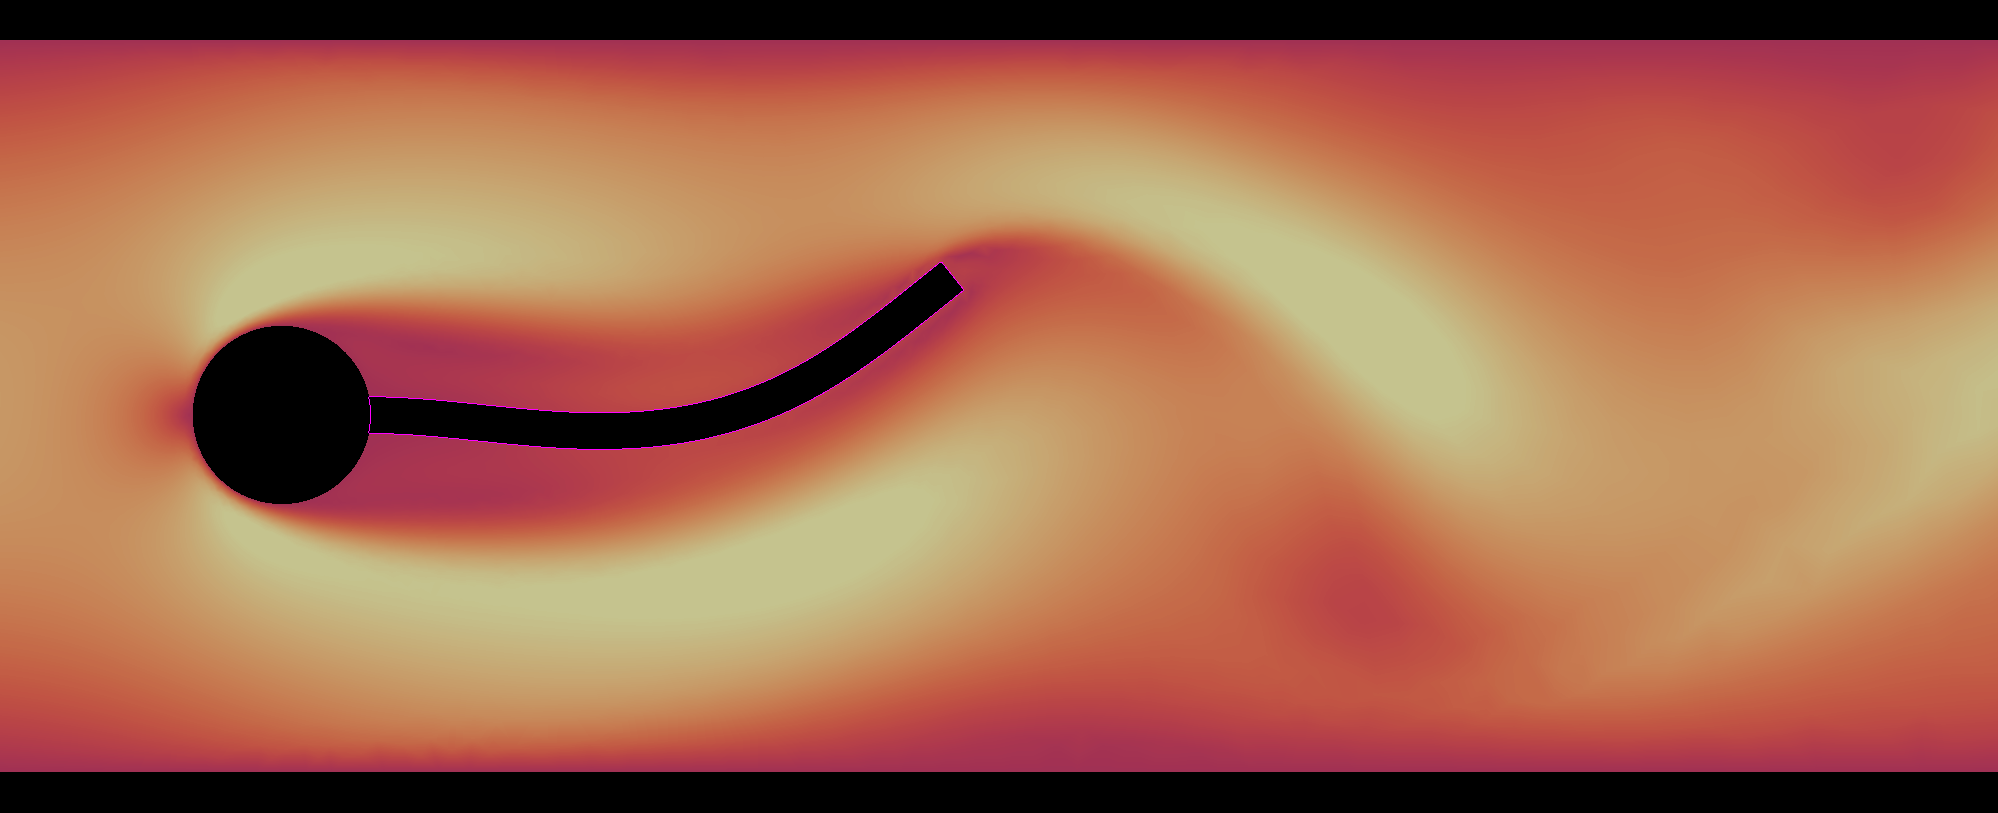
\includegraphics[scale=0.2]{./Fig/fsi2flow.png}
      \caption{FSI-2, visualization of fully developted flow with structure deformation at time t = 9s}
\end{figure}

\newpage
\subsubsection{FSI3}

\begin{table}[h!]
\centering
\caption{FSI 3 - Comparison of mesh extrapolation models}
\label{my-label}
\begin{tabular}{ |p{1cm}||p{1cm}|p{2.5cm}|p{2.5cm}|p{2.7cm}|p{2.7cm}|p{1.2cm}|}
 \hline
  \multicolumn{6}{|c|}{Laplace \hspace{2mm} $\Delta t = 0.01 \theta = 0.51$} \\
   \hline
nel & ndof & ux of A [x $10^{3}$]  &uy of A [x $10^{3}$]& Drag  & Lift \\
 \hline
 2474    & 21249  & -2.41      $\pm$ 2.41 & 1.49       $\pm$ 3.22 & 449.40       $\pm$ 14.70 & 0.55       $\pm$ 155.80  \\
 7307    & 63365  & -2.32       $\pm$ 2.30 & 1.34       $\pm$ 3.17 & 451.78       $\pm$ 16.08 & 1.13       $\pm$ 151.22  \\
 11556   & 99810  & -2.34       $\pm$ 2.34 & 1.57       $\pm$ 3.19 & 455.92       $\pm$ 17.32 & -0.10       $\pm$ 151.03 \\
 \hline
  \multicolumn{6}{|c|}{$\Delta t = 0.001 \theta = 0.501$} \\
   \hline
 nel & ndof & ux of A [x $10^{3}$]  &uy of A [x $10^{3}$]& Drag  & Lift \\
    \hline
1216 &5797& --2.17$\pm$  2.08 &     3.32     $\pm$  29.07 &439.98 $\pm$  14.08  &  1.91 $\pm$  151.71\\
2295 &10730& -3.04 $\pm$  2.88 &  1.51  $\pm$  35.88 & 452.04  $\pm$  22.41 &  3.30      $\pm$  160.11 \\
5963 &27486 & -3.03$\pm$  2.85 &  1.23 $\pm$  35.97  & 459.45  $\pm$  23.80 &  1.53  $\pm$  160.14 \\
 \hline
  \multicolumn{2}{|c|}{Reference}  & 136.7   & 10.53 & &\\
   \hline
    \multicolumn{2}{|c|}{Error}  & 0.007 \%   & 0.001 \% & &\\
   \hline
\end{tabular}
\end{table}

\begin{table}[h!]
\centering
%\caption{FSI 3 - Biharmonic BC1}
\label{my-label}
\begin{tabular}{ |p{0.9cm}||p{0.9cm}|p{2.49cm}|p{2.49cm}|p{2.6cm}|p{2.8cm}|}
 \hline
  \multicolumn{6}{|c|}{Biharmonic 1 \hspace{2mm}  $\Delta t = 0.01 \theta = 0.51$} \\
   \hline
nel & ndof & ux of A [x $10^{3}$]  &uy of A [x $10^{3}$]& Drag  & Lift \\
 \hline
 %2474    & 21249 & 7.96  $\pm$ 8.10  & -3.84   $\pm$ 1.02 & 450.16  $\pm$ 15.11 & $-20.09 \pm 148.17 $\\
 2474     &21249  &7.96  $\pm$ 8.10  &  -3.84   $\pm$ 1.02 & 450.16  $\pm$ 15.11  & -20.09 $\pm$ 148.17 \\
 7307    & 63365  & 3.10  $\pm$ 3.06  & -1.90   $\pm$ 4.21 & 457.37  $\pm$ 15.24 & -51.77 $\pm$ 127.28 \\
 11556   & 99810  & -2.18  $\pm$ 9.65 & 1.31    $\pm$ 4.93  & 456.40 $\pm$ 17.45 &  0.45 $\pm$ 149.68  \\
 \hline
  \multicolumn{6}{|c|}{$\Delta t = 0.001 \theta = 0.5$} \\
   \hline
 nel & ndof & ux of A [x $10^{3}$]  &uy of A [x $10^{3}$]& Drag  & Lift \\
1216 &5797  & -2.18       $\pm$ 2.10 & 3.56   $\pm$ 2.90 & 435.19       $\pm$ 9.77  & -1.57       $\pm$ 151.43 \\
7307    & 63365  & -1.42  $\pm$ 4.70 & 7.77   $\pm$ 2.85 & 454.38       $\pm$ 19.75 & 17.97       $\pm$ 155.08 \\
11556   & 99810  & -2.23  $\pm$ 6.16 & 1.72   $\pm$ 4.48 & 459.12       $\pm$ 22.97 & -3.12       $\pm$ 171.22 \\
 \hline
 \multicolumn{2}{|c|}{Reference} & -2.69 $\pm$  2.56                    & 1.48  $\pm$  34.38                   & 457.3  $\pm$  22.66        & 2.22  $\pm$- 149.78           \\
 \hline
 \multicolumn{2}{|c|}{Error}  & 0.007 \%   & 0.001 \% & &\\
 \hline
\end{tabular}
\end{table}

\begin{table}[h!]
\centering
%\caption{FSI 3 - Biharmonic BC2}
\label{my-label}
\begin{tabular}{ |p{1cm}||p{1cm}|p{2.5cm}|p{2.5cm}|p{2.7cm}|p{2.7cm}|p{1.2cm}|}
 \hline
  \multicolumn{6}{|c|}{Biharmonic 2 \hspace{2mm}  $\Delta t = 0.01 \theta = 0.51$} \\
   \hline
nel & ndof & ux of A [x $10^{3}$]  &uy of A [x $10^{3}$]& Drag  & Lift \\
 \hline
1216 &5797& -1.74  $\pm$  1.76 & 3.56 $\pm$  26.01 & 439.41$\pm$ 12.21  & -1.35    $\pm$  138.74\\
2295 &10730 & -2.39   $\pm$  2.40 &  1.76  $\pm$  32.27 & 449.71$\pm$ 18.16 &  3.71   $\pm$  149.97\\
 \hline
  \multicolumn{6}{|c|}{$\Delta t = 0.001 \theta = 0.501$} \\
   \hline
 nel & ndof & ux of A [x $10^{3}$]  &uy of A [x $10^{3}$]& Drag  & Lift \\
 1216 &5797& -3.39   $\pm$  3.38 &   1.23   $\pm$  36.61 &   413.26 $\pm$  51.82  &   57.19  $\pm$  222.65\\
 2295 &10730& -4.70  $\pm$  4.71& 1.49       $\pm$  44.62& 427.91$\pm$  93.17 &  44.38  $\pm$  268.05 \\
 \hline
 \multicolumn{2}{|c|}{Reference} & -2.69 $\pm$  2.56                    & 1.48  $\pm$  34.38                   & 457.3  $\pm$  22.66        & 2.22  $\pm$- 149.78           \\
 \hline
 \multicolumn{2}{|c|}{Error}  & 0.007 \%   & 0.001 \% & &\\
 \hline
\end{tabular}
\end{table}


\begin{figure}[h!]
    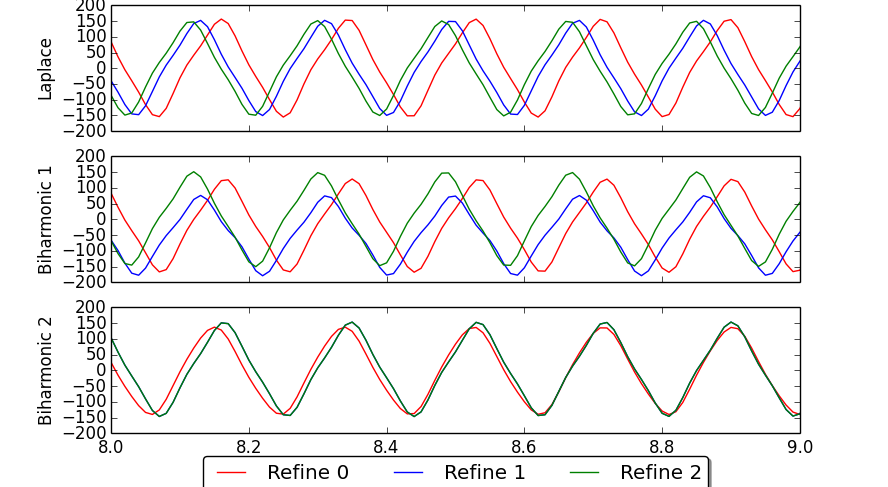
\includegraphics[scale=0.75]{./Fig/fsi3liftcompare.png}
      \caption{Comparing mesh extrapolation models}
\end{figure}

\begin{figure}[h!]
  \centering
    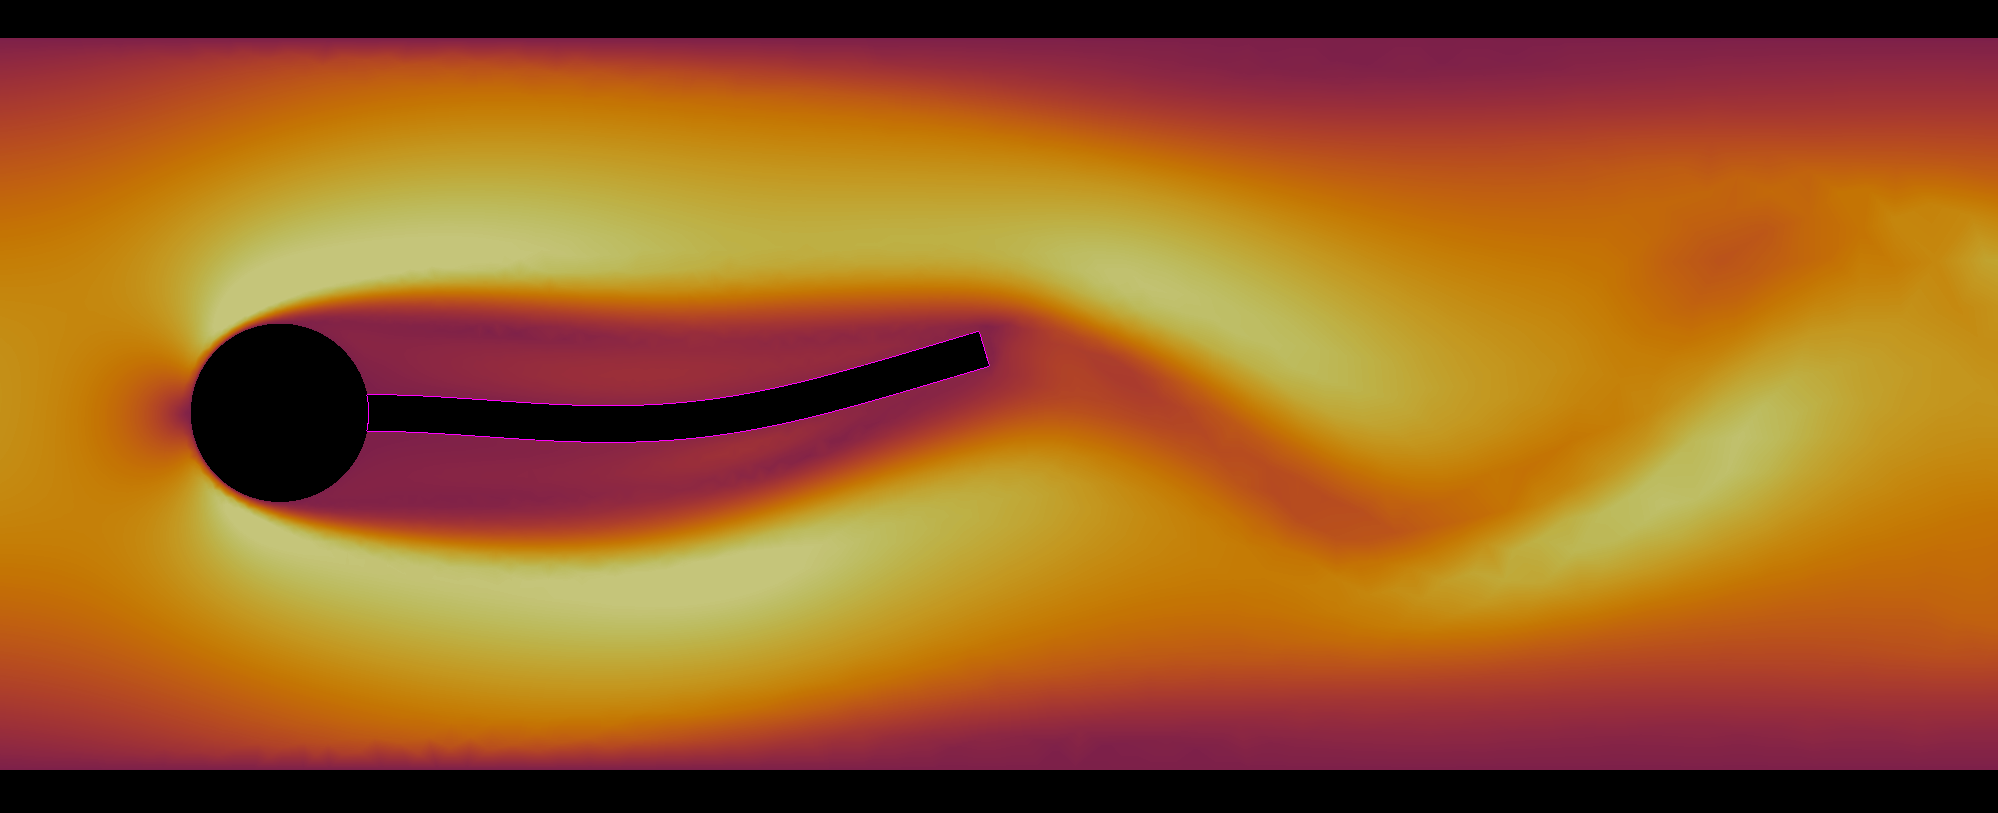
\includegraphics[scale=0.2]{./Fig/fsi3flow.png}
      \caption{FSI-3, visualization of fully developted flow with structure deformation at time t = 5.1s}
\end{figure}

\newpage
\subsection{Discussion of results}
Considering FSI1, all mesh extraplation models are of high accuracy compared to the reference solution.  However, due to the small deformations of order $10^{-6}$, FSI1 doesn't provide a rigorous test of the chosen mesh extrapolation model. By omitting mesh extrapolation from the variatonal formulation,  reasonable results are still obtained. This proves that the FSI-1 validation case can be misguiding, in terms of validating the chosen mesh extrapolation model. 

The FSI2 case proved to be one of the most demanding tests, due to the large deformation of the elastic flag. leading to the risk of entangled mesh cells. Therefore a high quality extrapolation of the solid deformation into the fluid is needed. All mesh extrapolation models proved to

The FSI3 environment does not induce deformation to the extent of the FSI2. However a critical phase in the transition to the periodic solution was discovered, where the pressure oscillation induces a large deformation to the system.

\section{Investigation of temporal stability}

Preliminary work regarding discretization and numerical analysis of Crank-Nicholson time stepping schemes for fluid structure interaction can be found in cite WIck papers. Two main properties of interest of higher-order methods have proven to be the stability of long-time simulation, and obtaining the expected physics for the problem of interest.

It is known that the Crank-Nicolson scheme can suffer from temporal stability, for long-term simulations \cite{Wick2013a}. Therefore,
the authors of \cite{Richter2015}, investigated temporal stability of the Crank-Nicolson scheme for the validation benchmark found in \cite{Hron2006}.  
The critera for the numerical experiements was to obatin a stable solution in the time interval [0, 10] minutes, by temporal and spatial refinement studies. The fully monolithic FSI problem discretized with second-order Crank-Nicolson, proved to give general stability problems for long-term simulation for certain time-steps \textit{k}. 

Following the ideas of \cite{Richter2015},, a second order scheme based on the Cranck-Nicholson yields two possibilities.
\begin{discr}
\textit{Crank–Nicolson secant method }
\begin{align*}
\Big[\frac{\ha{J}(\bat{u}^{n}) \bat{\nabla} \bat{v}^{n} \bat{F}_W^{-1}}{2} 
+ \frac{\ha{J}(\bat{u}^{n-1}) \bat{\nabla} \bat{}v^{n-1} \bat{F}_W^{-1}}{2} \Big] 
\frac{\bat{u}^{n} - \bat{u}^{n-1}}{k}
\end{align*} 
\end{discr}

\begin{discr}
\textit{Crank–Nicolson midpoint-tangent method}
\begin{align*}
\Big[\frac{\ha{J}(\bat{u}_{cn}) \bat{\nabla} \bat{v}_{cn} \bat{F}_W^{-1}}{2} \Big] 
\frac{\bat{u}^{n} - \bat{u}^{n-1}}{k} \hspace{4mm}
\bat{u}_{cn} = \frac{\bat{u}^{n} + \bat{u}^{n-1}}{2} \hspace{2mm}
\bat{v}_{cn} = \frac{\bat{v}^{n} + \bat{v}^{n-1}}{2}
\end{align*} 
\end{discr}

The numerical experiments showed very similar performance for Discretization 1.1 and 1.2 , and significant differences of temporal accuracy was not found. \\
Two options to coupe with the presented unstabilities are the \textit{shifted Crank-Nicolson} \cite{Richter2015}, \cite{Wicka}, \cite{Wick2013a},   and the \textit{frac-step method}. Both of these methods are defined as A-stable time-stepping schemes meaning..  In this thesis the shifted Crank-Nocolson scheme will be considered. \\
The shifted Crank-Nicolson scheme introduce further stability to the overall system, by shifting the $\theta$ paramter slightly to the implicit side. If the shift is dependent of the time-step \textit{k} such that $\frac{1}{2} \leq \theta \leq \frac{1}{2} + k$, the scheme will be of second order \cite{Richter2015}.

\newpage

\begin{figure}[h!]
 	\centering
    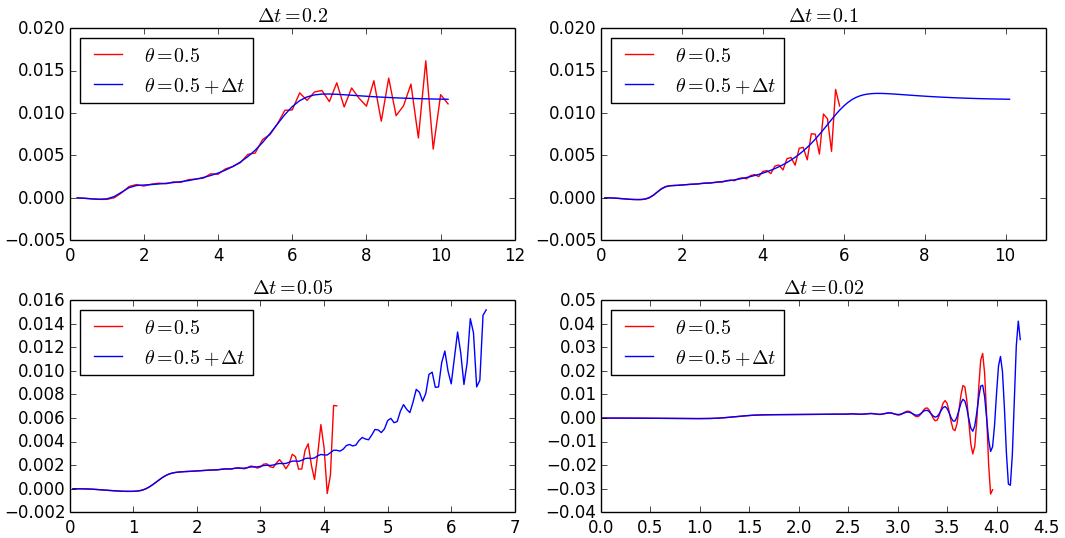
\includegraphics[scale=0.6]{./Fig/thetacheck.png} \\
    \vspace{2cm}
    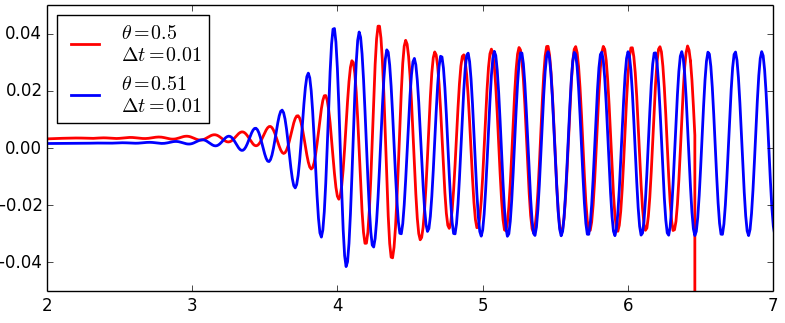
\includegraphics[scale=0.6]{./Fig/besttheta.png}
      \caption{Investigation of temporal stability for the FSI3 benchbark in the time interval $t \in [0, 10]$, comparing the shifted crank nicolson to the original cranc nicolson scheme. }
\end{figure}

A numerical investigation of temporal stability in shown in Table 1.7, where the shifted crank-nicolson scheme $\theta = 0.5 + k$, is compared the original crank-nicolson $\theta = 0.5$. The shifted version clearly show stability properties surpassing the original crank-nicolson scheme, for all numerical experiments. However, for $\Delta t \in [0.2, 0.1, 0.05, 0.02]$ the scheme clearly lacks the ability to capture the overall physics of the validation problem. Long-time stability and expected physical beavior is obtained for $\Delta t = 0.01$. However, numerical experiments showed that for $\Delta t \leq 0.005$ numerical stability was achieved regardless of both methods. This result is important, reducing the overall computational time needed to achieve reasonable accuracy.


\newpage
\section{Optimization of Newtonsolver}
A \textit{bottleneck} express a phenomena where the total performance of a complete implementation is limited to small code fragments, accounting for the primary consumption of computer resources.

As for many other applications, within computational science one can often assume the consummation of resources follows the \textit{The Pareto principle}. Meaning that for different types of events, roughly 80\% of the effects come from 20\% of the causes. An analogy to computational sciences it that 80\% of the computational demanding operations comes from 20\% of the code. In our case, the bottleneck is the newtonsolver. The two main reasons for this is 

\begin{itemize}
\item \textbf{Jacobian assembly} \\
The construction of the Jacobian matrix for the total residue of the system, is the most time demanding operations within the whole computation. 
\item \textbf{Solver}. \\ 
As iterative solvers are limited for the solving of fluid-structure interaction problems, direct solvers was implemented for this thesis. As such, the operation of solving a linear problem at each iteration is computational demanding, leading to  less computational efficient operations. Mention order of iterations?
\end{itemize}

Facing these problems, several attempts was made to speed-up the implementation. The FEniCS project consist of several nonlinear solver backends, were fully user-customization option are available. However one main problem which we met was the fact that FEniCS assembles the matrix of the different variables over the whole mesh, even though the variable is only defined in one to the sub-domains of the system.In our case the pressure is only defined within the fluid domain, and therefore the matrix for the total residual consisted of several zero columns within the structure region. FEniCS provides a solution for such problems, but therefore we were forced to construct our own solver and not make use of the built-in nonlinear solvers. \\

The main effort of speed-up were explored around the Jacobian assembly.
Of the speed-ups methods explored in this thesis, some are \textit{consistent} while others are \textit{nonconsistent}. Consistent methods are methods that always will work, involving smarter approaches regarding the linear system to be solved. The non-consistent method presented involves altering the equation to be solved by some simplification of the system. As these simplifications will alter the expected convergence of the solver, one must take account for additional Newton iterations against cheaper Jacobi assembly. Therefore one also risk breakdown of the solver as the Newton iterations may not converge.   


\subsection{Consistent methods}
\subsubsection{Jacobi buffering}
By inspection of the Jacobi matrix, some terms of the total residue is linear terms, and remain constant within each time step. By assembling these terms only in the first Newton iteration will save some assembly time for the additional iterations needed each time step. As consequence the convergence of the Newton method should be unaffected as we do not alter the system.  

\subsection{Non-consisten methods}    
\subsubsection{Reuse of Jacobian}
As the assembly of the Jacobian at each iteration is costly, one approach of reusing the Jacobian for the linear system was proposed. In other words, the LU-factorization of the system is reused until the Jacobi is re-assembled. This method greatly reduced the computational time for each time step. By a user defined parameter, the number of iterations before a new assembly of the Jacobian matrix can be controlled. 

\subsubsection{Quadrature reduce}
The assemble time of the Jacobian greatly depends on the degree of polynomials used in the discretisation of the total residual. Within FEniCS t he order of polynomials representing the Jacobian can be adjusted. The use of lower order polynomials reduces assemble time of the matrix at each newton-iteration, however it leads to an inexact Jacobian which may results to additional iterations. 


\subsection{Comparison of speedup methods}

\begin{figure}[h!]
 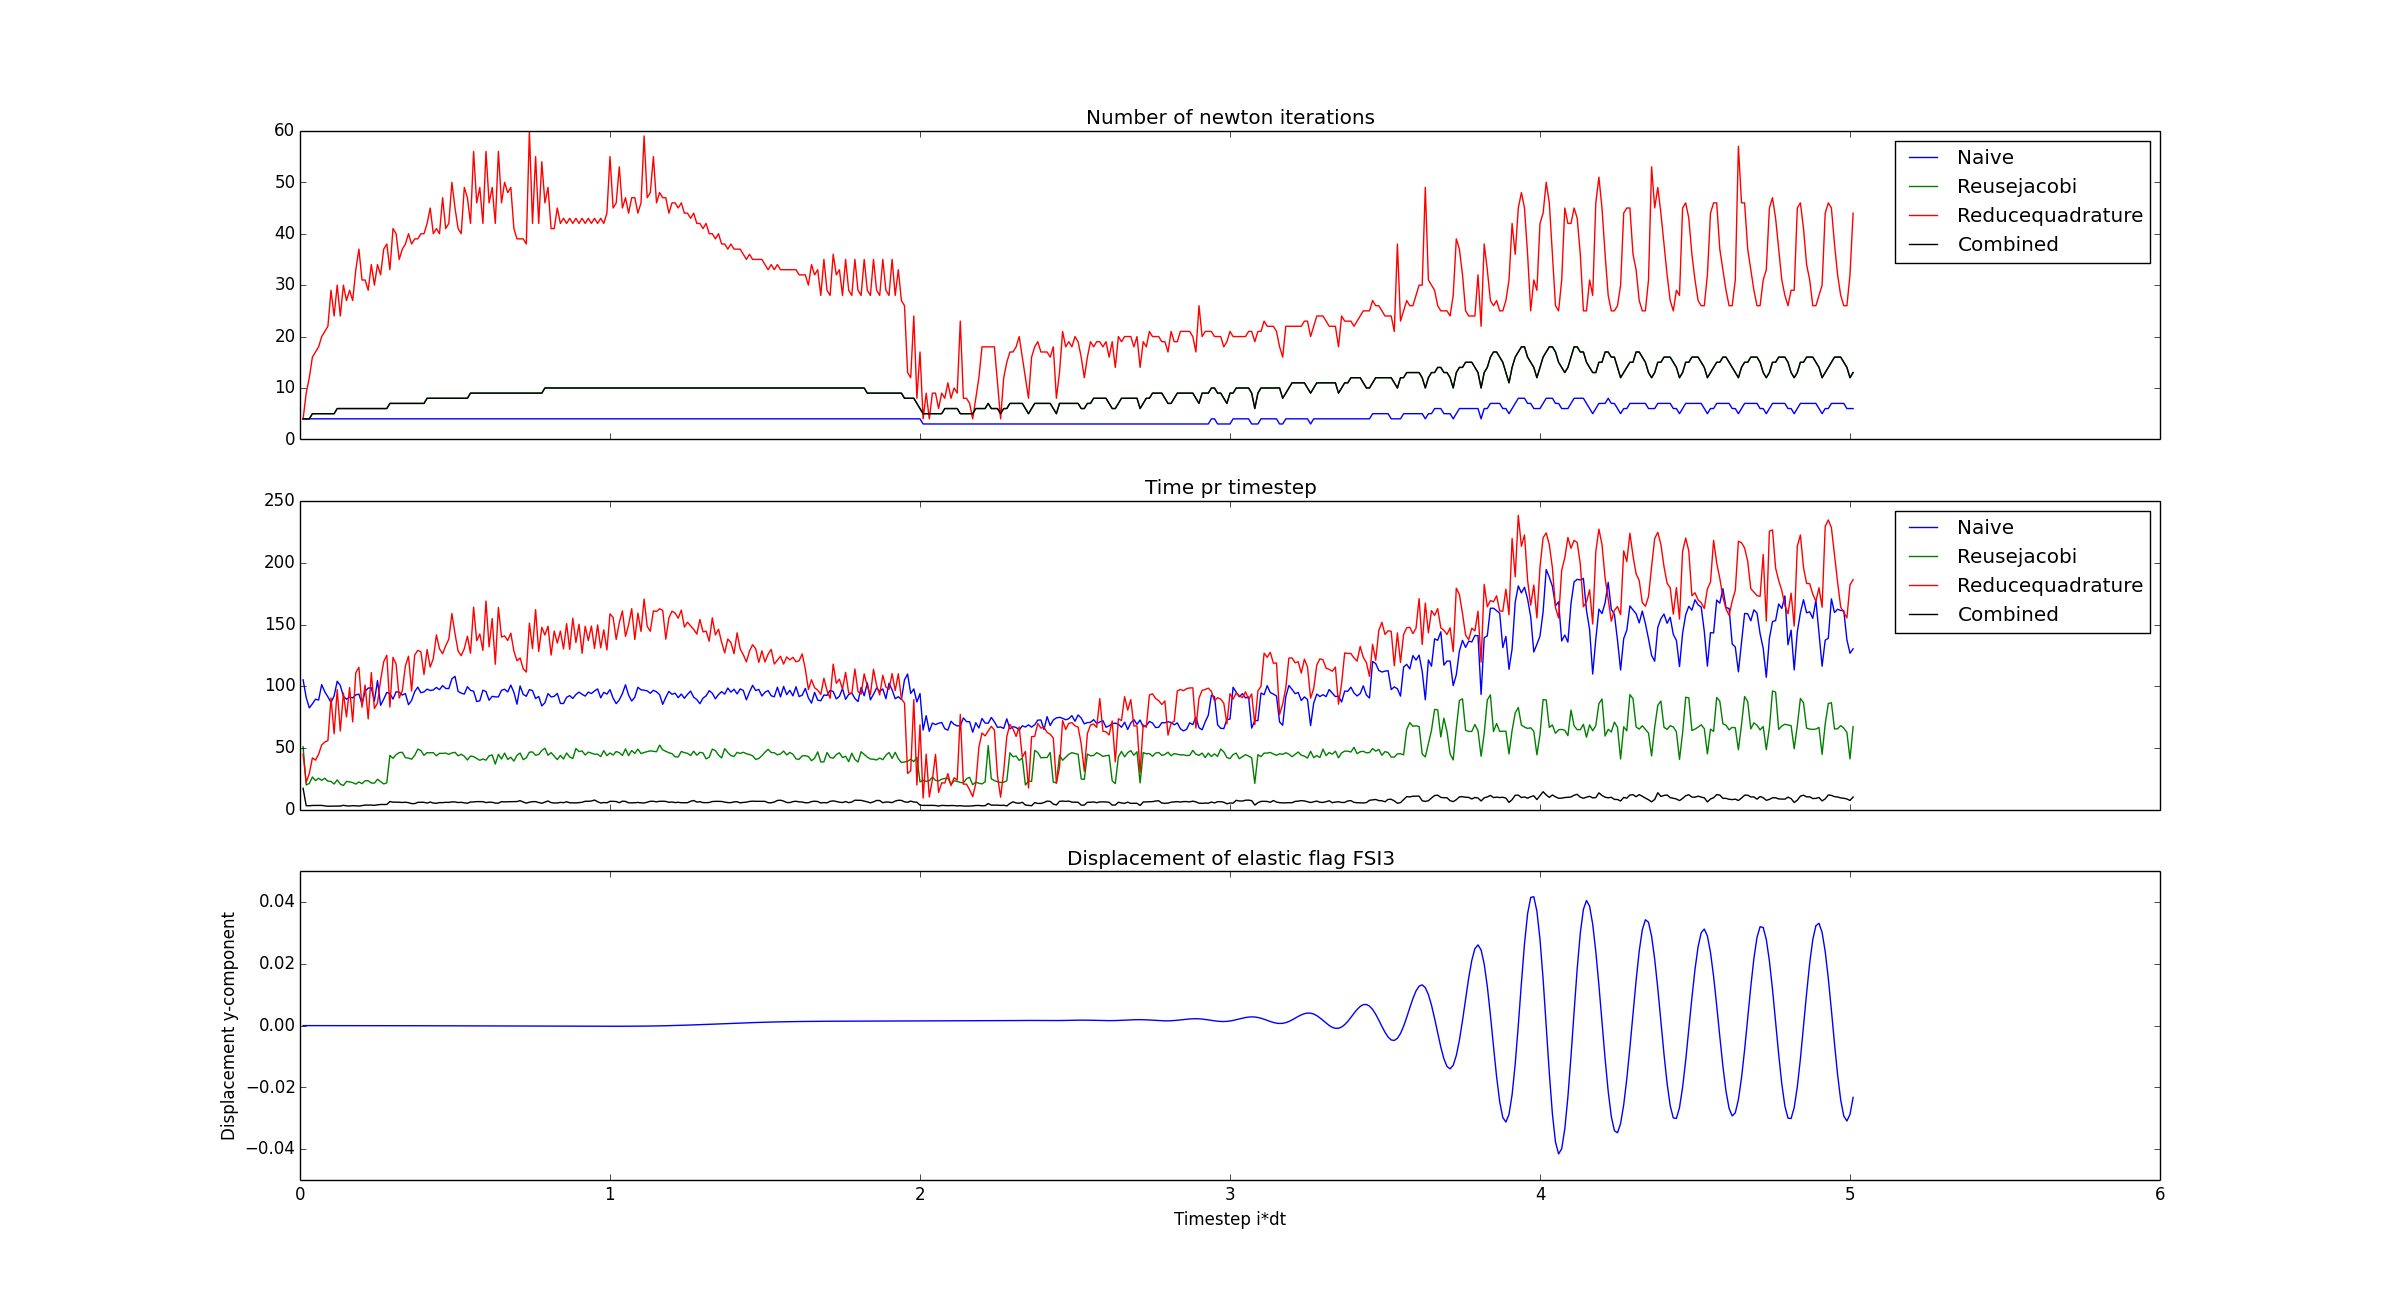
\includegraphics[scale=0.36]{./Fig/itercompare.png}
 \caption{Comparison of speed-up techniques for the laplace mesh model}
\end{figure}

\begin{figure}[h!]
 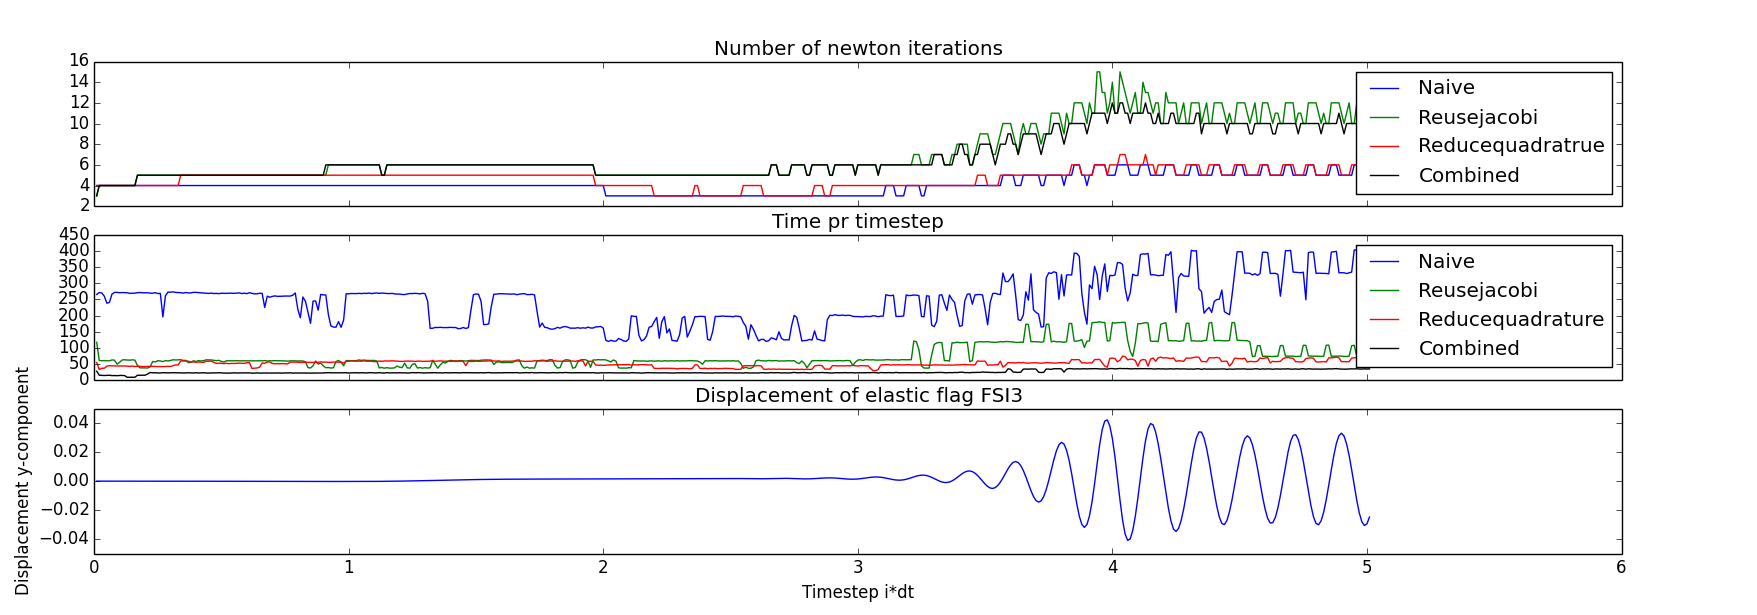
\includegraphics[scale=0.4]{./Fig/bi_compareit.png}
 \caption{Comparison of speed-up techniques for the biharmonic type 1 mesh model}
\end{figure}


\begin{table}[h!]
\centering
\caption{Comparison of speedup techniques}
\label{my-label}
\begin{tabular}{ |p{2.8cm}|p{2.2cm}|p{2.4cm}|p{2.4cm}|p{2.4cm}|p{2.4cm}| }
 \hline
  \multicolumn{6}{|c|}{Laplace} \\
 \hline
 Implementation       &Naive  & Buffering & Reducequad. & Reusejacobi & Combined \\
 \hline
 Mean time/timestep &  123.1    &  &  31.4 & 61.3  &  11.1 \\
 \hline
 Speedup \%            &  1.0         &  & 74.46\%     &  50.19\%     & 90.97 \%   \\
 \hline 
 Mean iteration         &  4.49       &  & 10.1  &  10.2  &  10.2 \\
 \hline 
  \hline
  \multicolumn{6}{|c|}{Biharmonic Type 1} \\
 \hline
 Implementation &Naive  & Buffering & Reducequad. & Reusejacobi & Combined \\
 \hline
 Mean time/timestep & 243.3 & 307.6  & 51.6 & 76.7  &  24.8 \\
 \hline
 Speedup \%    & 1.0     & -26\% & 78.7\%  & 68.4 \%  &  89.7\%   \\
 \hline
 Mean iteration & 4.1     &  6.2    &4.6&  7.1 &  6.8  \\
 \hline
  \hline
  \multicolumn{6}{|c|}{Biharmonic Type 2} \\
 \hline
 Implementation &Naive  & Buffering & Reducequad. & Reusejacobi & Combined \\
 \hline
 Mean time/timestep &        &            &   60.5   &   95.3     &  20.7  \\
 \hline
 Speedup \%             & 1.0  & \%     & \%          &  \%         &  \%   \\
 \hline
 Mean iteration           & 4.1 &           &  6.29     &   6.9        &  6.9  \\
 \hline 
\end{tabular}
\end{table}

